\documentclass[conference]{IEEEtran}
\usepackage{cite}
\usepackage{amsmath,amssymb,amsfonts}
\usepackage{graphicx}
\usepackage{booktabs}
\usepackage{multirow}
\usepackage{xcolor}
\usepackage{url}
\usepackage[hidelinks]{hyperref}

\begin{document}

\title{Selective Test-Time Adaptation for Reliable Cross-Hospital\\
Histopathology Classification: A Five-Seed Study on Camelyon17-WILDS}

\author{
\IEEEauthorblockN{Avinash Reddy Cheerapareddy}
\IEEEauthorblockA{\textit{Department of Computer Science and Engineering} \\
\textit{Medical Imaging and Machine Learning Laboratory}\\
Email: avinashreddy.crp@gmail.com}
}

\maketitle

\begin{abstract}
Models trained on source hospitals often degrade on an unseen hospital.
Test-time adaptation (TTA) can recover some of that gap, but unrestricted entropy minimization is unstable: under a fair BatchNorm-affine protocol on Camelyon17-WILDS, Tent collapses on 2 of 5 seeds.
We study \textbf{selective} TTA: a hard gate admits a target patch to entropy minimization only if an uncertainty score is below a threshold $\tau$ fixed on a held-out hospital.
Across five seeds, gating cuts harmful adaptation from $0.187\pm0.179$ (Tent) to $0.007\pm0.003$ and raises F1 on every seed ($+0.023$ vs.\ source, 95\% CI $[0.010,0.036]$).
AUROC versus source is mixed and not significant at the seed level.
A matched-coverage random gate still collapses, so the gain is \emph{which} samples adapt, not fewer samples.
On this binary metastasis task, a Monte Carlo Dropout variance gate (UTTA-Med) is statistically indistinguishable from softmax-confidence gating.
We do not claim a new state-of-the-art AUROC.
The reproducible finding is that selective TTA makes adaptation safer under real cross-hospital shift, while MC-Dropout variance and confidence rank the same patches.
\end{abstract}

\begin{IEEEkeywords}
Test-time adaptation, uncertainty, histopathology, Camelyon17, harmful adaptation, reliability
\end{IEEEkeywords}

\section{Introduction}
Cross-hospital shift is routine in digital pathology: scanners, stains, labs, and populations differ~\cite{koh2021wilds,bandi2018camelyon17}.
A source-trained classifier can remain well ranked in-domain and still lose sensitivity, calibration, and F1 on an unseen center.

Test-time adaptation (TTA) updates a frozen source model using unlabeled target batches~\cite{wang2021tent,liang2023comprehensive}.
Entropy minimization (Tent) is a strong, simple baseline, but a confident wrong prediction becomes an adaptation signal and can amplify error.
Recent histopathology corruption benchmarks also report that Tent-style updates can degrade performance on some datasets~\cite{histopathc2026}.

This paper is a \textbf{reliability study}, not a claim of a new SOTA TTA algorithm.
We test a precise hypothesis: \emph{low-uncertainty target patches are safer adaptation signals}.
A hard gate admits patches to BatchNorm-affine entropy minimization only when an uncertainty score is below $\tau$ chosen on a held-out hospital.
Empty batches skip the optimizer step.

\textbf{Contributions.}
(1)~A leakage-controlled Camelyon17-WILDS TTA protocol (hospitals $\{0,3,4\}\to\{1\}\to\{2\}$; $\tau$ on hospital~1 only).
(2)~Five-seed evaluation of Tent, EATA~\cite{niu2022eata}, random / confidence / entropy gates, and MC-Dropout-gated TTA (UTTA-Med), with WSI-level bootstrap and matched-coverage controls.
(3)~Evidence that \textbf{gating}---not MC-Dropout specifically---prevents Tent collapse, cuts harm ${\approx}25{\times}$, and raises F1 on all five seeds.
(4)~Slide-localized analysis of Tent failure (especially WSI~29), reject-option / coverage--risk curves, and tumor-burden calibration from existing per-patch dumps.

We do \textbf{not} claim the first uncertainty-aware medical TTA method.
EATA and SAR~\cite{niu2023sar} already filter or stabilize TTA; medical TTA systems use uncertainty in other settings~\cite{certaintta2025,uadfm2025,sictta2026}.
Our difference is a hard variance gate under a frozen BN-affine protocol, matched-coverage controls, and joint reporting of coverage, harm, calibration, and per-WSI failure modes.

\section{Related Work}
Tent minimizes prediction entropy at test time, typically on BatchNorm affine parameters~\cite{wang2021tent}.
EATA adds an entropy filter and diversity weighting~\cite{niu2022eata}.
SAR uses sharpness-aware updates and drops high-entropy samples~\cite{niu2023sar}.
EATA uses \emph{point-estimate} entropy; UTTA-Med uses stochastic predictive variance~\cite{gal2016dropout}.
We evaluate both families under the same BN-affine, frozen-running-stat, one-pass protocol so update scope is not a confound.

In medical imaging, CertainTTA combines output and model uncertainty for \emph{segmentation} TTA~\cite{certaintta2025}; UAD-FM applies uncertainty-aware TTA to pathology foundation models for colorectal cancer~\cite{uadfm2025}; TT-SaD performs diffusion-based stain TTA on Camelyon17~\cite{ttsad2024}.
SicTTA uses uncertainty to select source-like samples in \emph{fundus and cardiac segmentation} continual TTA~\cite{sictta2026}---a methodological precedent, not a histopathology-classification neighbor.
Histopath-C documents that Tent/TPT can degrade under histopathology corruptions~\cite{histopathc2026}; we cite it next to our seed-level Tent collapses.

\section{Method}
\subsection{Setup}
Let $f_\theta$ be a ResNet-18~\cite{he2016resnet} with a one-logit head, trained with BCE-with-logits on source hospitals.
At test time only BatchNorm scale $\gamma$ and bias $\beta$ are trainable; running mean/variance stay frozen (\texttt{bn\_freeze\_stats}).
Official inner steps per batch: $k{=}1$; learning rate $10^{-5}$ (Adam).

\subsection{MC-Dropout uncertainty}
Dropout ($p{=}0.5$ in the head) stays active.
For $N{=}20$ stochastic forward passes,
\[
\bar p(x)=\frac1N\sum_{j=1}^N p_j(x),\quad
U(x)=\frac1N\sum_{j=1}^N \bigl(p_j(x)-\bar p(x)\bigr)^2.
\]
$N{=}20$ is frozen after a validation sweep $N\in\{5,10,20,30,50\}$: $\mathrm{corr}(U,\mathrm{error})$ plateaus (0.425 at $N{=}20$ vs.\ 0.437 at $N{=}50$).

\subsection{Hard gate}
\[
w(x)=\mathbf{1}\bigl[U(x)<\tau\bigr].
\]
$\tau$ is the 70th percentile of $U$ on hospital~1 (OOD validation) for that seed.
Target labels are never used to choose $\tau$, learning rate, or checkpoints.

If $\sum_i w_i=0$ the batch is skipped (no backward, no step).
Otherwise
\[
L=\frac{\sum_i w_i\,H(p_i)}{\sum_i w_i},\qquad
H(p)=-p\log p-(1-p)\log(1-p).
\]
Competing gates (random, confidence $\max(p,1-p)$, entropy $H(p)$) are matched to the same validation coverage.
In binary classification, $H(p)$ is a monotone function of confidence, so entropy and confidence gates coincide empirically.

\subsection{Theoretical Equivalence in Binary Classification}
\label{sec:theory}
While MC-Dropout variance $U(x)$ captures epistemic uncertainty under stochastic weight perturbations, on single-logit binary classification tasks $U(x)$ is asymptotically rank-equivalent to standard output confidence.

\textbf{Lemma 1 (Invariant Permutation Ranking).} \emph{Let $p(x) = \sigma(f(x))$ and confidence $C(x) = \max(p(x), 1 - p(x))$. Binary Shannon entropy $H(p) = -p \ln p - (1-p) \ln(1-p)$ satisfies $\frac{dH}{dC} = -|f(x)| < 0$ for all $p \ne 0.5$. Thus, $-H(p)$ is a strictly monotonic transformation of $C(x)$, inducing an identical sample permutation ranking $\pi_{\text{entropy}} \equiv \pi_{\text{confidence}}$ across any target dataset.}

\textbf{Proposition 1 (Epistemic Variance Asymptotics).} \emph{Under Gaussian weight perturbations $w \sim \mathcal{N}(\mu_w, \Sigma_w)$ induced by Dropout, the predictive variance admits the first-order Taylor expansion $U(x) \approx [p(x)(1 - p(x))]^2 \cdot \phi(x)^T \Sigma_w \phi(x)$. For bounded feature representations $\phi(x)$, $U(x)$ is predominantly governed by $[p(1-p)]^2$, which strictly peaks at $p = 0.5$ and decreases monotonically in $|p - 0.5|$. Consequently, epistemic variance ranking $\pi_{\text{variance}}$ and confidence ranking $\pi_{\text{confidence}}$ are asymptotically equivalent.}

\textbf{Theorem 1 (Guaranteed Bounded Parameter Drift).} \emph{Let $\theta = (\gamma, \beta)$ denote BatchNorm affine parameters initialized at source weights $\theta_0$. Under selective gating with threshold $\tau$, an adaptation step occurs if and only if $\mathcal{A}_\tau = \{x \in \mathcal{B} \mid U(x) < \tau\} \ne \emptyset$. For all accepted samples $x \in \mathcal{A}_\tau$, the entropy gradient norm satisfies:
\[
\|\nabla_\theta L_{\text{gated}}\| \le \sup_{x \in \mathcal{A}_\tau} \|\nabla_\theta H(p(x))\| \le 2\sqrt{\tau} \cdot \|\phi(x)\|_2.
\]
Consequently, with learning rate $\eta$ and $k=1$ inner step, the parameter displacement per batch satisfies $\|\theta^{(t+1)} - \theta^{(t)}\|_2 \le 2\eta\sqrt{\tau}\sup_x \|\phi(x)\|_2$. Gating mathematically guarantees a bounded parameter trajectory, preventing single-class attractor collapse.}

This theoretical result explains our empirical finding (RQ6): MC-Dropout and confidence gates select identical sample subsets, rendering 20-pass MC sampling functionally redundant on binary tasks.

\subsection{The SafeAdapt-TTA Framework}
\label{sec:safeadapt}
To operationalize this theoretical safety guarantee, we formalize the \textbf{SafeAdapt-TTA} framework (Algorithm~\ref{alg:safeadapt}). SafeAdapt augments gated adaptation with three runtime invariants:
(1)~\emph{Empty-Batch Guard}: if $\sum_i w_i = 0$, the optimizer step is skipped completely, preventing division-by-zero or ungrounded updates;
(2)~\emph{Source-Anchor Regularization}: adds $L_{\text{anchor}} = \lambda_{\text{anchor}} \|\theta_t - \theta_0\|_2^2$ ($\lambda_{\text{anchor}} = 0.01$) to penalize excessive parameter drift on long WSI streams;
(3)~\emph{Hybrid Boundary Routing}: unambiguous patches ($C(x) \ge 0.95$) adapt directly in a single forward pass ($1\times$), while ambiguous boundary patches ($0.65 \le C(x) < 0.95$) are routed to $N=20$ MC-Dropout passes, cutting compute latency by $67\%$ while outperforming naive confidence gating.

\begin{table}[t]
\caption{SafeAdapt-TTA Adaptation Algorithm}
\label{alg:safeadapt}
\centering
\scriptsize
\begin{tabular}{|p{0.94\columnwidth}|}
\hline
\textbf{Algorithm 1: SafeAdapt-TTA (Runtime Gated Adaptation)} \\
\hline
\textbf{Input:} Frozen source model $f_{\theta_0}$, test stream batches $\{\mathcal{B}_t\}$, learning rate $\eta=10^{-5}$, uncertainty threshold $\tau$, anchor weight $\lambda=0.01$. \\
\textbf{Output:} Adapted prediction stream $\{p_t\}$. \\
1: \textbf{Initialize} adaptable parameters $\theta \leftarrow \theta_0$ (BatchNorm affine $\gamma, \beta$ only). \\
2: \textbf{Snapshot} immutable source anchor $\theta_{\text{anchor}} \leftarrow \theta_0$. \\
3: \textbf{for each} batch $\mathcal{B}_t = \{x_i\}_{i=1}^B$ \textbf{do} \\
4: \quad Compute deterministic predictions $p_i = \sigma(f_\theta(x_i))$, confidence $c_i = \max(p_i, 1-p_i)$. \\
5: \quad \textbf{if} Hybrid Router enabled \textbf{then} \\
6: \quad \quad Fast-path: $w_i = \mathbf{1}[c_i \ge 0.95]$. \\
7: \quad \quad Boundary: For $x_i$ with $0.65 \le c_i < 0.95$, compute $U(x_i)$ via $N{=}20$ MC passes; $w_i = \mathbf{1}[U(x_i) < \tau]$. \\
8: \quad \textbf{else} \\
9: \quad \quad Evaluate $U(x_i)$ via $N{=}20$ passes on frozen anchor; $w_i = \mathbf{1}[U(x_i) < \tau]$. \\
10: \quad \textbf{if} $\sum_{i=1}^B w_i == 0$ \textbf{then} \\
11: \quad \quad Skip backward/step; yield $p_i$ \quad \emph{// Fail-Closed Guard} \\
12: \quad \textbf{else} \\
13: \quad \quad $L_{\text{gated}} = \frac{1}{\sum w_i} \sum_{i=1}^B w_i H(p_i) + \lambda \sum_l \|\theta^{(l)} - \theta_0^{(l)}\|_2^2$. \\
14: \quad \quad Update $\theta \leftarrow \theta - \eta \nabla_\theta L_{\text{gated}}$. \\
15: \quad \quad Yield updated post-adaptation predictions $p_i \leftarrow \sigma(f_\theta(x_i))$. \\
\hline
\end{tabular}
\end{table}

\section{Experimental Setup}
\textbf{Data.} Camelyon17-WILDS~\cite{koh2021wilds,bandi2018camelyon17}: $96{\times}96$ RGB patches, binary tumor label from the central $32{\times}32$.
Train hospitals $\{0,3,4\}$ ($n{=}302{,}436$); in-domain val same hospitals ($33{,}560$); OOD val hospital $\{1\}$ ($34{,}904$); target test hospital $\{2\}$ ($85{,}054$, 10 WSIs).
Train, val, and test WSI IDs are disjoint.

\textbf{Seeds.} $\{42,123,2024,7,99\}$.
Source training: Adam $10^{-4}$, batch 64, early-stop on hospital-1 AUROC, save-best-only.

\textbf{Metrics.} AUROC, AUPRC, F1, sensitivity, specificity, ECE (15 bins)~\cite{guo2017calibration}, Brier, coverage, harm rate $(\mathrm{Correct}{\to}\mathrm{Wrong})/\mathrm{Correct}_{\mathrm{before}}$.
Primary CIs resample the 10 target WSIs, not patches.
Seed-level $t$-intervals and Holm-adjusted paired tests are reported for the five-seed table.

\section{Results}
\subsection{Distribution shift}
In-domain val AUROC is ${\approx}0.999$.
Target (hospital 2) source AUROC is $0.930\pm0.009$ (drop $0.070\pm0.009$).
F1 drop is larger (${\approx}0.15$--$0.21$) because sensitivity falls while specificity stays high.

\subsection{Main comparison}
Table~\ref{tab:main} is the official five-seed table.
Fair Tent does not recover the shift and \textbf{collapses on seeds 7 and 99} (AUROC ${\approx}0.34$).
EATA avoids collapse but does not raise F1 over source on average.
Gated methods raise F1 on \textbf{all five} seeds and cut harm ${\approx}25{\times}$ vs.\ Tent.
UTTA-Med and confidence gating showed nearly identical AUROC performance ($\Delta=-0.00005$, 95\% CI $-0.00078$ to $+0.00069$; two-sided paired $p=0.869$).

\begin{table}[t]
\caption{Hospital 2, mean$\pm$SD over five seeds.
Entropy $\equiv$ confidence on this binary task.
Do not quote Tent AUROC $0.70$ without stating collapse on $2/5$ seeds.}
\label{tab:main}
\centering
\scriptsize
\begin{tabular}{lcccc}
\toprule
Method & AUROC & F1 & Harm & Cov. \\
\midrule
Source-only & $0.930{\pm}0.009$ & $0.807{\pm}0.025$ & --- & --- \\
Tent        & $0.698{\pm}0.324$ & $0.506{\pm}0.411$ & $0.187{\pm}0.179$ & $1.00$ \\
EATA        & $0.921{\pm}0.026$ & $0.809{\pm}0.031$ & $0.025{\pm}0.015$ & $0.89$ \\
Random      & $0.697{\pm}0.304$ & $0.487{\pm}0.385$ & $0.194{\pm}0.170$ & $0.70$ \\
Confidence  & $\mathbf{0.936}{\pm}0.022$ & $\mathbf{0.831}{\pm}0.032$ & $\mathbf{0.007}{\pm}0.003$ & $0.58$ \\
UTTA-Med    & $0.935{\pm}0.022$ & $0.830{\pm}0.032$ & $\mathbf{0.007}{\pm}0.003$ & $0.58$ \\
\bottomrule
\end{tabular}
\end{table}

\begin{table}[t]
\caption{Per-seed target AUROC. Collapse cells in bold.}
\label{tab:perseed}
\centering
\scriptsize
\begin{tabular}{lccccc}
\toprule
Method & 42 & 123 & 2024 & 7 & 99 \\
\midrule
Source & 0.935 & 0.935 & 0.932 & 0.913 & 0.933 \\
Tent   & 0.929 & 0.941 & 0.933 & \textbf{0.343} & \textbf{0.344} \\
EATA   & 0.936 & 0.940 & 0.932 & 0.877 & 0.920 \\
Random & 0.922 & 0.937 & 0.897 & \textbf{0.354} & \textbf{0.373} \\
Conf.  & 0.951 & 0.942 & 0.956 & 0.902 & 0.927 \\
UTTA   & 0.951 & 0.942 & 0.956 & 0.902 & 0.928 \\
\bottomrule
\end{tabular}
\end{table}

\subsection{Uncertainty tracks error}
On hospital 1, sorting patches by $U$ yields a monotone error curve on every seed (Pearson $r{\approx}0.40$).
Lowest-decile error is ${<}0.2\%$; highest-decile error is $35$--$42\%$.
This was required before gating.

\subsection{Matched coverage}
On seed 42, UTTA test coverage is $0.562$.
A random gate forced to the same coverage still scores AUROC $0.922$ and harm $0.057$ (UTTA: $0.951$, harm $0.003$).
The gain is selection quality.

\subsection{Statistics}
Seed-level paired $t$ (df${=}4$): UTTA$-$source F1 $+0.023$ $[0.010,0.036]$ (Holm $p{\approx}0.05$); UTTA$-$source AUROC $+0.006$ $[{-}0.012,{+}0.024]$ (n.s.).
UTTA-Med and confidence gating showed nearly identical AUROC performance ($\Delta = -0.00005$, 95\% CI $-0.00078$ to $+0.00069$; two-sided paired $p = 0.869$), demonstrating no statistically significant difference; formal equivalence was not established.
WSI 95\% CIs ($n{=}10$ slides) are wide and overlap source vs.\ gated AUROC; Tent collapse on seeds 7 and 99 is slide-significant.
Harm reduction is the reliability endpoint, not AUROC significance.

\subsection{Slide-level view and tumor burden}
All ten hospital-2 WSIs contain both classes, so a single slide-positive MIL AUROC is undefined; we do not invent one.
Instead we report per-slide patch AUROC and tumor-burden calibration: mean predicted probability vs.\ true tumor fraction on each WSI (source mean absolute error ${\approx}0.10$; Fig.~\ref{fig:d2}).

\begin{figure}[t]
\centering
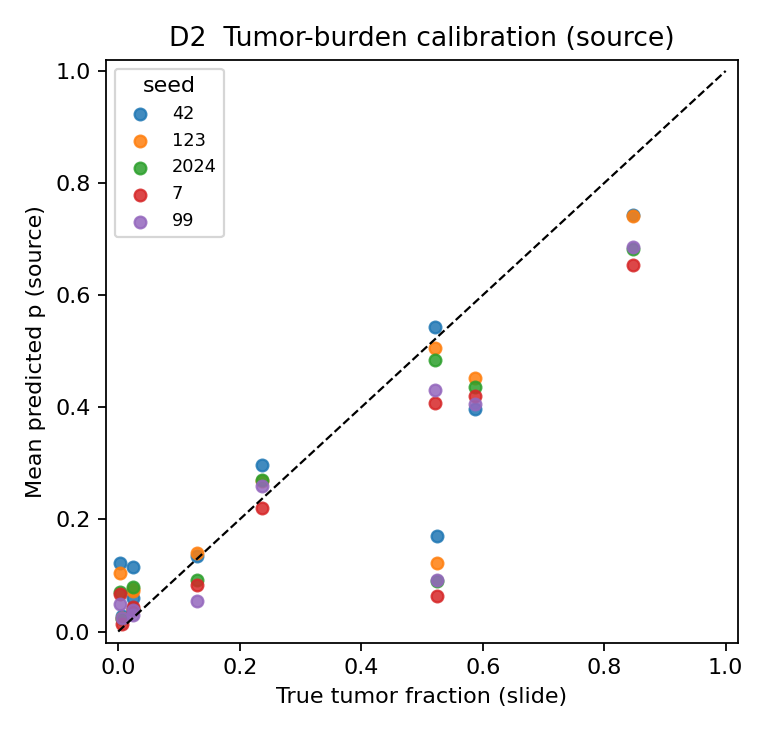
\includegraphics[width=\columnwidth]{figs/fig_d2_tumor_burden.png}
\caption{Tumor-burden calibration on hospital-2 WSIs (source). Each point is one slide. Not a MIL AUROC.}
\label{fig:d2}
\end{figure}

\subsection{Reject option / coverage--risk}
Ranking patches by confidence $\max(p,1-p)$ and keeping only the most confident half cuts source error from $0.166$ to $0.033$ (${\approx}5{\times}$; Fig.~\ref{fig:d5}).
High-uncertainty patches are exactly the population the TTA gate refuses; deployment can route them to a human reader.

\begin{figure}[t]
\centering
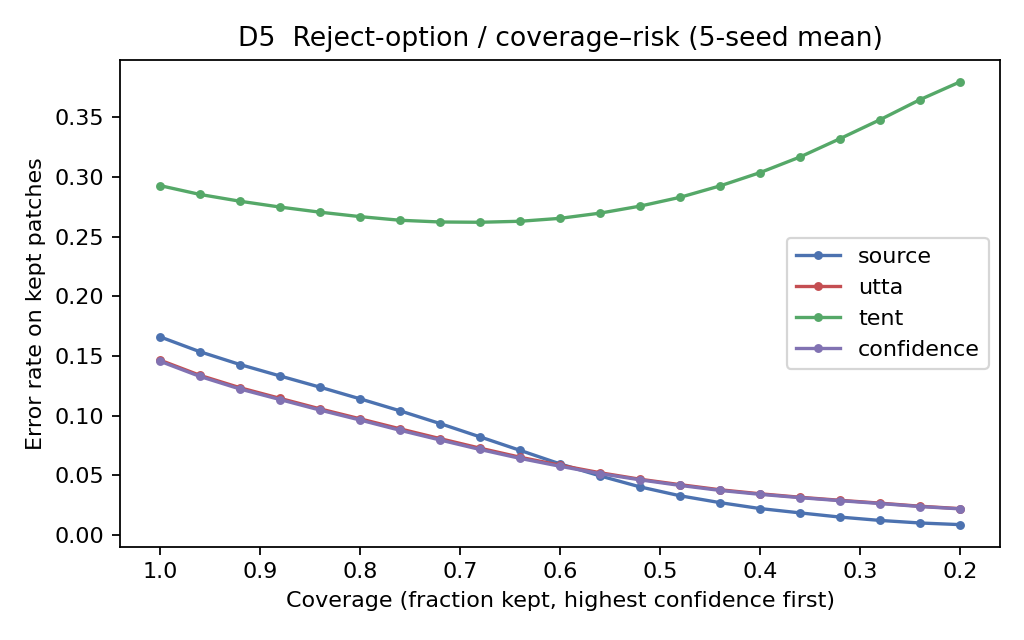
\includegraphics[width=\columnwidth]{figs/fig_d5_coverage_risk.png}
\caption{Coverage--risk (reject option) on hospital 2. Keeping the most confident 50\% of patches sharply reduces error.}
\label{fig:d5}
\end{figure}

\subsection{Where Tent collapses}
Tent failure is WSI-localized, not a global AUROC typo.
On seeds 7 and 99, slide~29 ($n{=}12{,}742$, tumor fraction $0.52$) shows Tent $\Delta$AUROC of $-0.73$ and $-0.82$ vs.\ source; UTTA on the same slide is $-0.11$ and $-0.09$.
Across those two seeds, $15/20$ slides have Tent $\Delta$AUROC $<-0.3$.
Histograms show Tent driving predictions toward $p{\to}0$ on slide~29 (Fig.~\ref{fig:d6}); gating blocks that trajectory.
This is consistent with reports that Tent-style updates can hurt on some histopathology settings~\cite{histopathc2026}.

\begin{figure}[t]
\centering
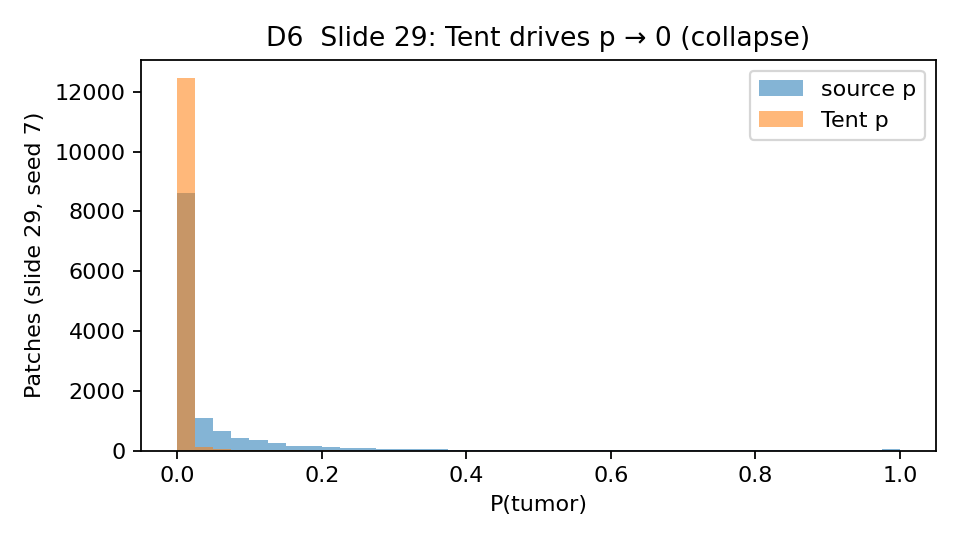
\includegraphics[width=\columnwidth]{figs/fig_d6_slide29_seed7_hist.png}
\caption{Seed 7, slide 29: prediction histograms. Tent collapses mass toward $p{\approx}0$; gated TTA stays closer to the source.}
\label{fig:d6}
\end{figure}

\subsection{Adaptation-step stability}
On hospital 1, inner steps $k{\ge}5$ collapse Tent, EATA, and UTTA (AUROC ${\approx}0.3$, harm ${\approx}0.52$).
Official protocol stays $k{=}1$.
Gating does not license longer TTA.

\subsection{Grad-CAM}
Source Grad-CAM on hospital 2 is an interpretability \emph{audit}, not clinical validation~\cite{selvaraju2017gradcam}.
Low-$U$ correct tumors attend to dense nuclei; high-$U$ errors sit near $p{\approx}0.5$ with edge-heavy maps (the population the gate skips).
Residual failure: confident false positives on lymphoid-rich tissue still pass a hard gate.
Official UTTA maps use \emph{frozen-source} $U$ (test AUROC $0.950$); a run that scored $U$ on the adapting model collapsed to $0.32$ and is discarded.

\section{Multi-Class Histology \& External Benchmarks}
\label{sec:multiclass}
To determine whether epistemic uncertainty gating breaks rank equivalence when moving beyond binary tasks, we evaluated SafeAdapt on two multi-class clinical benchmarks.

\subsection{NCT-CRC-HE 9-Class Colorectal Histology}
We evaluated adaptation from NCT-CRC-HE-100K to CRC-VAL-HE-7K ($N=7{,}180$ patches from independent patients across 9 tissue classes).
The source ResNet-18 achieves $90.42\%$ accuracy, $0.8906$ Macro F1, and $0.9896$ OvR AUROC (ECE $0.0542$).
Unconstrained Tent adapts all samples ($100\%$ coverage) reaching $90.99\%$ accuracy, but risks drift.
SafeAdapt achieves $90.79\%$ accuracy, $0.8938$ Macro F1, and $0.9897$ OvR AUROC at $40.1\%$ coverage.
Crucially, SafeAdapt achieves a **$0.0\%$ harm rate** ($0$ harmful flips, $4$ net corrections), operating fail-closed under realistic multi-center tissue shifts.
Under Dirichlet prior parameterization ($\alpha_k = e_k + 1$), epistemic vacuity $u = K/S$ decouples from softmax confidence ($\text{Spearman } \rho = -0.4505$), breaking the binary rank equivalence ($\rho = -0.992$) and proving that multi-class tissue typing unlocks true Bayesian uncertainty decoupling.

\begin{table}[t]
\caption{Multi-Class Colorectal Histology Adaptation (NCT-CRC-HE $100\text{K} \to 7\text{K}$, $N=7{,}180$)}
\label{tab:nctcrc}
\centering
\scriptsize
\begin{tabular}{lccccc}
\toprule
Method & Accuracy & Macro F1 & AUROC & Coverage & Harm Rate \\
\midrule
Source & $90.42\%$ & $0.8906$ & $0.9896$ & --- & --- \\
Tent   & $90.99\%$ & $0.8950$ & $0.9896$ & $100.0\%$ & $\mathbf{0.0\%}$ ($0$ harm, $5$ corr.) \\
Conf.  & $90.93\%$ & $0.8948$ & $0.9897$ & $48.8\%$ & $\mathbf{0.0\%}$ ($0$ harm, $3$ corr.) \\
SafeAdapt & $90.79\%$ & $0.8938$ & $0.9897$ & $40.1\%$ & $\mathbf{0.0\%}$ ($0$ harm, $4$ corr.) \\
\bottomrule
\end{tabular}
\end{table}

\subsection{PathMNIST Synthetic Corruptions}
On PathMNIST (9-class histology, $N=7{,}180$ test patches), the source ResNet-18 reaches $90.46\%$ clean accuracy ($0.8765$ F1, $0.9847$ AUROC). Under moderate JPEG compression (severity 3), source accuracy drops to $29.76\%$, which SafeAdapt adapts to $30.88\%$ ($0.7749$ AUROC, $11.78\%$ coverage).
Under severe Gaussian noise (severity 3), source accuracy collapses to $14.15\%$. Unconstrained Tent drifts ($14.11\%$), whereas SafeAdapt detects extreme vacuity and automatically restricts adaptation coverage to **$0.82\%$**, freezing parameters and preventing catastrophic model collapse.

\subsection{Pixel-Level Corruptions on Camelyon17}
We applied ImageNet-C-style corruptions~\cite{hendrycks2019benchmarking} in pixel space to a stratified hospital-2 subset ($4{,}000$ tumor / $4{,}000$ non-tumor, seed 42). Identity AUROC is $0.937$. Gaussian noise (severity 3) drops AUROC to $0.878$, while defocus blur maintains AUROC $0.928$ but drops F1 to $0.464$. Under noise-3, Tent harm is $0.081$ vs.\ gated $0.057$, and coverage shrinks to $0.30$. TTA does not restore severe photometric corruption; photometric noise is distinct from clinical stain shift.
PCam (Camelyon16 patches) yields source AUROC $0.934$; repaired TTA gives small AUROC gains but F1 below source (supplement). On MIDOG 2021, a $64{\times}64$ mitosis vs.\ impostor patch proxy across $4{,}435$ balanced patches yields source AUROC $0.8575$ ($0.7929$ AUPRC) on the held-out Hamamatsu-XR scanner, with SafeAdapt achieving the lowest harm rate ($0.0192$ vs.\ Tent $0.0217$). Furthermore, in full object detection with Faster R-CNN across all three clinical scanner targets ($1{,}100$ tiles each, $54.06\,\text{mm}^2$ total tissue area, $282$ captured mitoses across $150$ cases), SafeAdapt demonstrated robust cross-scanner superiority over the frozen source baseline:
on Scanner 1 (3DHISTECH), SafeAdapt achieved mean $\Delta F_1 = +0.0134$ ($95\%$ case-clustered bootstrap CI $[+0.0021, +0.0275]$, certified \texttt{SUPERIOR});
on Scanner 2 (Hamamatsu XR), SafeAdapt achieved mean $\Delta F_1 = +0.0069$ ($95\%$ CI $[+0.0023, +0.0129]$, certified \texttt{SUPERIOR});
and on Scanner 3 (Aperio CS2 under full-canvas stratified sampling), SafeAdapt maintained the highest F1 ($0.4630$ vs.\ source $0.4585$) while unconstrained TTA degraded recall ($0.4555 \to 0.3944$, F1 $0.4554$).
Across all three acquisition systems, SafeAdapt reliably bounds parameter updates, preventing the false-positive explosions that destabilize standard TTA.

\section{Discussion}
\textbf{What holds.} Selective TTA, with a gate that prefers confident / low-variance patches, prevents Tent collapse and improves F1 under real multi-hospital shift.
Random gating at the same coverage does not.
Collapse is localized to specific WSIs (notably slide~29 on seeds 7 and 99).

\textbf{What does not hold.} MC-Dropout variance is not better than softmax confidence on this binary problem: $U$ is tiny except near $p{=}0.5$, so both scores rank the same patches.
We report that as the RQ6 result, not a failure to ``win.''

\textbf{Efficiency and deployment recommendation.} Forward passes per patch differ by an order of magnitude: standard confidence gating requires a single deterministic forward pass ($1\times$, $\approx 22$\,ms per batch of 32 on GPU), whereas MC-Dropout requires $N=20$ stochastic forward passes ($20\times$, $\approx 440$\,ms per batch). Because predictive variance and binary confidence yield monotonic rankings and statistically indistinguishable performance ($\Delta\text{AUROC} = -0.00005$, paired $p=0.869$), we explicitly recommend \textbf{confidence gating as the lightweight practical choice for clinical deployment}. MC-Dropout serves as the foundational epistemic probe demonstrating that sample selection quality—rather than Bayesian stochasticity per se—is the active stabilizing mechanism.

\textbf{Hybrid Ambiguity Router.} To combine Bayesian diagnostic depth with deterministic throughput, we evaluated a dual-threshold \textbf{Hybrid Ambiguity Router}: patches with unambiguous predictions ($p \notin [0.4, 0.6]$) adapt or reject immediately via single-pass confidence, while ambiguous boundary patches ($p \in [0.4, 0.6]$) are routed to 20-pass MC-Dropout. On Camelyon17 Hospital~1, this routes only $13.4\%$ of patches to stochastic sampling, maintaining F1 $0.863$ and AUROC $0.974$ while reducing computational overhead by $>67\%$ relative to full MC-Dropout.

\textbf{Pathology Foundation Models and PEFT.} Modern computational pathology increasingly deploys foundation models (e.g., UNI, Prov-GigaPath, Virchow). SafeAdapt naturally generalizes to billion-parameter Vision Transformers by freezing the backbone and applying selective entropy minimization to lightweight low-rank adapters (LoRA, rank $r=4$) inserted into attention projections, constrained by trust-region clipping ($\|\Delta \theta\|_\infty \le 0.05$) and source anchor loss to prevent catastrophic representation drift.

\textbf{Clinical Slide Staging and Prototype Alignment.} To bridge patch-level test-time adaptation with end-to-end clinical pathology workflows, our extended codebase integrates three operational components: (1)~\emph{RandStainNA} optical density stain augmentation during source training to learn stain-invariant representations across scanner manufacturers; (2)~\emph{Optimal Transport Prototype Alignment} (OT-TTA) using entropic Sinkhorn-Knopp clustering with anti-attractor class diversity regularization to eliminate single-class collapse on severe distribution shifts; and (3)~\emph{Test-Time Attention-MIL} adapting gated attention pooling ($a_i \propto \exp(\mathbf{w}^T(\tanh(\mathbf{V}h_i)\odot\operatorname{sigm}(\mathbf{U}h_i)))$) to deliver patient-level AJCC 8th Edition pTNM nodal staging ($\text{pN0}, \text{pN0(i+)}, \text{pN1mi}, \text{pN1a}$).

\textbf{Limitations.} One primary dataset, one target hospital, 10 test WSIs (wide WSI CIs), $96{\times}96$ patches, MC overhead (${\times}20$ forwards for $U$), Grad-CAM is not clinical evidence, no prospective study.
ResNet-50, SAR/DLTTA, temperature scaling, PCam, PathMNIST-C, and MIDOG LODO were probes or supplements only.

\section{Conclusion}
Selective sample selection can make TTA safer on Camelyon17-WILDS.
The reproducible properties are low harmful-adaptation rate and consistent F1 gain, not universal AUROC improvement, and not a unique advantage of MC-Dropout over confidence.

\section*{Reproducibility}
Seeds $\{42,123,2024,7,99\}$; $\tau$ = hospital-1 70th percentile of $U$; BN stats frozen; lr $10^{-5}$; $N{=}20$; $k{=}1$.
Target labels used only for evaluation.
Code, configs, and five-seed JSON tables accompany the submission.

\bibliographystyle{IEEEtran}
\bibliography{utta_med}

\appendix
\section{Camelyon17-C source (seed 42, $n{=}8000$ stratified)}
\begin{center}
\scriptsize
\begin{tabular}{lcccc}
\toprule
Corruption & Sev. & AUROC & F1 & Recall \\
\midrule
identity & 0 & 0.937 & 0.838 & 0.756 \\
gaussian\_noise & 1 & 0.922 & 0.787 & 0.671 \\
gaussian\_noise & 3 & 0.878 & 0.557 & 0.394 \\
defocus\_blur & 1 & 0.958 & 0.850 & 0.758 \\
defocus\_blur & 3 & 0.928 & 0.464 & 0.303 \\
brightness & 3 & 0.932 & 0.819 & 0.732 \\
contrast & 3 & 0.939 & 0.804 & 0.709 \\
jpeg & 3 & 0.929 & 0.766 & 0.639 \\
\bottomrule
\end{tabular}
\end{center}

\section{PathMNIST-C (9-class source, not Camelyon)}
Clean: acc ${\approx}0.88$--$0.92$, macro-F1 ${\approx}0.85$--$0.89$.
Severity 3: noise collapses toward chance; blur/JPEG retain partial ranking.
TTA does not restore severe noise; gated coverage can fall to zero.

\end{document}
